% 2008 年新课标卷理科第 1 题：y=2sin(ωx+φ)（ω>0）在 [0,2π] 上的图象。
% 来源 PDF：gaokaomath-src/普通高考/2008/2008新课标理(海南,宁夏).pdf
% SHA-256：e16be52b93c241bf45c4d6441855b577407007de032d2e902f11442c06ef66ec
% 原页：2008新课标理(海南,宁夏).pdf 第 1 页（A3 三栏）第 1 栏，书页码 467。
% 绘制依据：按原页图象在 [0,2π] 上恰含 2 个周期、起点在原点，即 y=2sin 2x；
%   x 轴标注刻度 1 与终点 2π，y 轴标注 1。
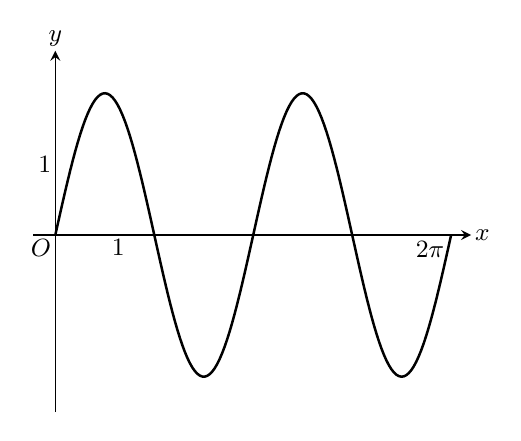
\begin{tikzpicture}[x=0.8cm, y=0.9cm, semithick, every node/.style={inner sep=1.2pt, font=\small}]
  \draw[->,>=stealth] (-0.35,0) -- (6.6,0) node[right] {$x$};
  \draw[->,>=stealth] (0,-2.5) -- (0,2.6) node[above] {$y$};
  \node[below left] at (0,0) {$O$};
  \node[below] at (1,0) {$1$};
  \node[below left=1pt] at (6.283,0) {$2\pi$};
  \node[left] at (0,1) {$1$};
  \draw[domain=0:6.283, samples=160, line width=0.9pt] plot (\x, {2*sin(2*\x r)});
\end{tikzpicture}
